\documentclass[a4paper,12pt]{article}
\usepackage[utf8]{inputenc}

%  Русский язык
\usepackage{multirow}
\usepackage{wrapfig}
\usepackage[T2A]{fontenc}			% кодировка
\usepackage[utf8]{inputenc}			% кодировка исходного текста
\usepackage[english,russian]{babel}	% локализация и переносы

\usepackage{indentfirst} %Красная строка
\usepackage[a4paper,top=1.3cm,bottom=2cm,left=1.5cm,right=1.5cm,marginparwidth=0.5cm]{geometry}
\usepackage[usenames]{color}
\usepackage{colortbl}
\usepackage{csvsimple}
\usepackage{siunitx}



% Заметки
\usepackage{todonotes}

% Математика
\usepackage{amsmath,amsfonts,amssymb,amsthm,mathtools} 
\usepackage{hyperref}

\renewcommand{\AA}{\ensuremath{\mathring{A}}}

\begin{document}
\def\figurename{Рисунок}
\begin{titlepage}
\begin{center}
    {\large МОСКОВСКИЙ ФИЗИКО-ТЕХНИЧЕСКИЙ ИНСТИТУТ (НАЦИОНАЛЬНЫЙ ИССЛЕДОВАТЕЛЬСКИЙ УНИВЕРСИТЕТ)}
\end{center}
\begin{center}
    {\largeФизтех-школа биологической и медицинской физики}
\end{center}

\vspace{1cm}
{\huge
\begin{center}
    {\bf Лабораторная работа по физической химии}\\
    \vspace{0.5cm}
    Свойства электродов
\end{center}
}

\vspace{4cm}
\begin{flushright}
{\LARGE Выполнила студентка группы Б06-103:\\ Фитэль Алена \\}

\end{flushright}
\vspace{9cm}
\begin{center}
    Долгопрудный, 2023 г.
\end{center}
\end{titlepage}
\newpage
\section{Введение}


\textbf{Цели и задачи работы:}
\begin{itemize}
\item Знакомство с понятием лимитирующей стадии электрохимической реакции и
двумя принципиально разными причинами изменения потенциала электрода в
условиях протекания тока – при быстрой и медленной электрохимической стадии
\item Особые требования к элементам трехэлектродной схемы при исследовании
вольт-амперных характеристик протекающих реакций
\item  Получение хлорсеребряного электрода и изучение его свойств.
\item  Исследование свойств платинового электрода в условиях его поляризуемости и
обратимости. Оценка ключевых параметров диффузионной и кинетической
стадий электрохимических реакций. 
\end{itemize}
\section{Теоретический материал}
\subsection{Поляризуемые и неполяризуемые электроды}
    
\underline{Идеально поляризуемым(необратимым) электродом} называется тот, у которого сопротивление стадии переноса заряда велико, поэтому в интервале потенциалов, когда ток заряжения больше тока электрохимической реакции, электрод эквивалентен конденсатору. Всё вприкладываемое напряжение идёт на зпряжение ДЭС электрода.\\
\underline{Идеально неполяризуемый(обратимый) электрод} - электрод с малым сопротивлением стадии переноса заряда, он находится в равновесии с продуктами электрохимической реакции. При подаче напряжения на электрод, возникает электрическое поле, которое вызывает ток, в свою очередь сбрасывающий "лишний" заряд. 
\subsection{Трёхэлектродная электрохимическая ячейка}
    
\begin{figure}[h!]
    \centering
    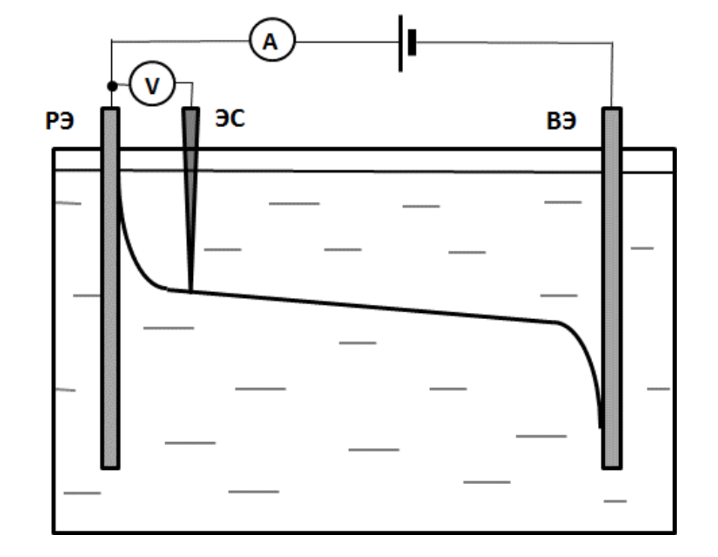
\includegraphics[width = 0.4\textwidth]{трёхЭ_схема.png}
    \caption{Трёхэлектродная электрохимическая ячейка}
    \label{fig:no_int}
\end{figure}\\
    
Ячейка включает в себя \underline{рабочий электрод(РЭ)} - исследуемый электрод. \underline{электрод срав-}\
\underline{нения(ЭС)}, который должен быть идеально неполяризуемым, его потенциал постоянен и определяется только концентрацией потенциалоопределяющих ионов. ЭС подключается в цепь с высокоточным милливольтметром с очень большим сопротивлением. Чтобы минимизировать омическое падение напряжения в растворе, ЭС располагают близко к РЭ. Для уменьшения диффузионного скачка потенциала и повышения точности работы ЭС его подключают к РЭ через тонкий капилляр и солевой мостик. Ещё один электрод ячейки - \underline{вспомогательный электрод(ВЭ)}, он не должен лимитировать измеряемую величину, поэтому $S_{\text{РЭ}} \ll S_{\text{ВЭ}}$. Так же ВЭ должен быть отделён пористой перегородкой от остального раствора, чтобы продукты реакции на этом электроде не попадали в рабочий раствор.\\
При протекании тока электрохимической реакции, между электродами возникает разность потенциалов:
\[ U = E_0 + |\Delta{E_{\text{РЭ}}}| + |\Delta{E_{\text{ВЭ}}}| + IR_{\text{цепи}} \]
где $E_0$ - ЭДС источника, $\Delta{E}$ - электрохимические поляризации электродов, $IR_{\text{цепи}}$ - омическое падение напряжения в растворе.\\
Учитывая все указанные выше детали, трёхэлектродная электрохимическая ячейка позволяет измерять потенциал РЭ точностью до потенциала ЭС.\\
\subsection{Многостадийность прохождения электрического тока}
    
Поляризуемость или неполяризуемость электрода определяется величиной активационного барьера и скоростью кинетической стадии переноса заряда на электроде. Так же активационный барьер влияет на ВАХ при протекании тока. Электродная реакция, протекающая на границе раздела фаз, приводящая к возникновению тока, включает в себя несколько последовательных стадий:

\begin{figure}[h!]
    \centering
    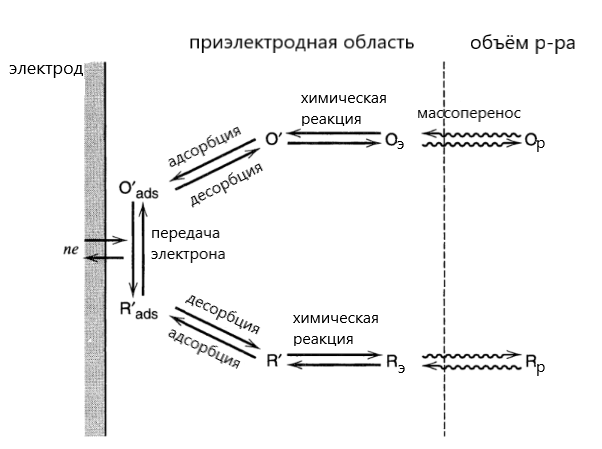
\includegraphics[width = 0.5\textwidth]{стадии_тока.png}
    \caption{Стадии прохождения электродной реакции на границе раздела фаз}
    \label{fig:no_int}
\end{figure}\\

Самая медленная стадия будет определять скорость всего процесса, в данном случае величину тока.\\
\subsection{Диффузионно-лимитированный процесс и концентрационная поляризация}
Рассмотрим неполяризуемый электрод, для которого кинетическая стадия реакции проходит быстро, тогда лимитирует процесс массоперенос реагентов из раствора. Подача реагентов обусловлена конвекцией, диффузией или миграцией. В глубине раствора за счёт конвекции и мешалок концентрация остаётся постоянной, однако вблизи электрода существует \underline{неперемешиваемый(диффузионнный) слой}, в котором возникает градиент концентрации, этот слой находится непосредственно за дифуузной частью ДЭС, где восстанавливается электронейтральность раствора.\\
Из-за разности поверхностной(непосредственно за диффузной частью ДЭС) и объёмной(в глубине раствора) концентрации возникает явление, называемое \underline{концентрационной поляри-}\\
\usepackage{зацией} - это значит, что на электроде возникает потенциал, отклоняющийся от равновесного(при отсутствии градиента концентрации):
\[ \eta = E - E_p = E^0 + \frac{RT}{nF}\ln{c_i^s} - \frac{RT}{nF}\ln{c_i^b} = \frac{RT}{nF}\ln{\frac{c_i^s}{c_i^b}} \]
где $\eta$ - перенапряжение из-за градиента концентрации, E - потенциал электрода, $E_p$ - равновесный потенциал электрода, $c_i^s$ и $c_i^b$ - концентрации на поверхности и в объёме соответственно.\\

Введём понятие \underline{предельного диффузионного тока} - максимальный диффузионный ток, достигаемый при $c_i^s$ = 0:
\[ i_d = -nFD\frac{c_i^b}{\delta} \]
где D - коэффициент диффузии, $\delta$ - толщина неперемешиваемого слоя.\\
Это выражение получено в предположении, что диффузия стационарна, поэтому концентрация в диффузионном слое меняется линейно.\\

Получим, что $\frac{c_i^s}{c_i^b} = 1 - \frac{i}{i_d}$, тогда получим ВАХ  для ситуации, когда только катодные процессы лимитируются диффузией:
\[ i = i_d[1 - exp(\frac{nF\eta}{RT})] \]

\begin{figure}[h!]
    \centering
    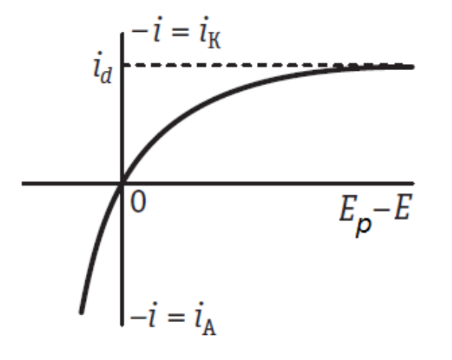
\includegraphics[width = 0.4\textwidth]{ВАХ_к.png}
    \caption{Зависимость тока от концентрационной поляризации при разряде ионов металла на одноимённом металле}
    \label{fig:no_int}
\end{figure}\\

Из графика видно, что катодный процесс лимитирован диффузией и этот ток стремится к своему предельному значению, анодный процесс в данном случае не затруднён диффузией, поэтому ток растёт неограничено.\\


Из графика видно, что катодный процесс лимитирован диффузией и этот ток стремится к своему предельному значению, анодный процесс в данном случае не затруднён диффузией, поэтому ток растёт неограничено.\\

Так выглядит зависимость перенепряжения от тока, когда и окислитель и восстановитель требуют диффузии из раствора:
\[ E - E_p = \frac{RT}{nF}\ln{(1 - \frac{i}{i_d^{(O)}})} - \frac{RT}{nF}\ln{(1 - \frac{i}{i_d^{(R)}})} \]
где $i_d^{(O)}$ и $i_d^{(R)}$ - предельные диффузионные токи окисленной и восстановленной форм

\begin{figure}[h!]
    \centering
    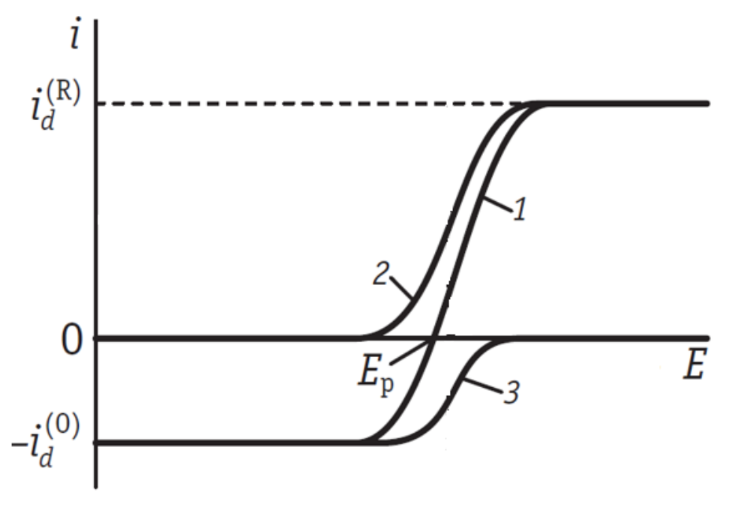
\includegraphics[width = 0.4\textwidth]{ВАХ_к_а.png}
    \caption{ВАХ процесса, в котором и окисление и восстановление лимитированны диффузией}
    \label{fig:no_int}
\end{figure}\\

где 2 и 3 - ток восстановленной и окисленной формы соответсвенно, а 1 - суммарный ток\\

\subsection{Кинетические закономерности стадии переноса электрона}
    
Рассмотрим границу области поляризуемости идеально поляризуемого электрода, для которого кинетическая стадия переноса заряда является лимитирующей.\\

Любую электрохимическую реакцию можно представить в виде:
\[ Ox + ne = Red \]
Или иначе на языке зарядов:
\[ Z_O - n = Z_R \]
Заметим, что:
\[ E = E_p \Rightarrow i^{\to} = i^{\leftarrow} = i_0 \] где $i_0$ - \underline{ток обмена}
\[ E > E_p \Rightarrow i_A = i^{\leftarrow} - i^{\to} \]
\[ E < E_p \Rightarrow i_K = i^{\to} - i^{\leftarrow} \]
Пусть все электроны в реакции переносятся в одну стадию, а энергия активации катодного и анодного процесса линейно связаны с потенциалом электрода: $E_a(Red) = \alpha{E}, E_a(Ox) = \beta{E}; \alpha + \beta = 1$, тогда вблизи электрода из уравнения Аррениуса для преимущественно превращения Red в Ox и при $i = i^{\leftarrow} - i^{\to}$ получим [уравнение Батлера-Фольмера]:
\[ i = i_0[exp(\frac{nF\alpha\eta}{RT}) - exp(-\frac{nF(1 - \alpha)\eta}{RT})] \]


при $\eta \gg \frac{RT}{nF} \simeq 25\text{мВ} \Rightarrow i \simeq i_0exp(\frac{nF\alpha\eta}{RT})$, тогда пусть $a = -\frac{RT}{nF\alpha}\ln{i_0}, b = 2,3\frac{RT}{nF\alpha}\ln{i_K}$, получаем [формулу Тафеля]:
\[ \eta = a +b\lg{i} \]

при $\eta \ll \frac{RT}{nF} \simeq 25\text{мВ} \Rightarrow E \to E_p$; $\eta \simeq \frac{RT}{nF}\frac{i}{i_0} = \Theta{i}$,
где $\Theta$- сопротивление стадии переноса заряда.

\begin{figure}[h!]
\begin{center}
\begin{minipage}[h!]{0.45\linewidth}
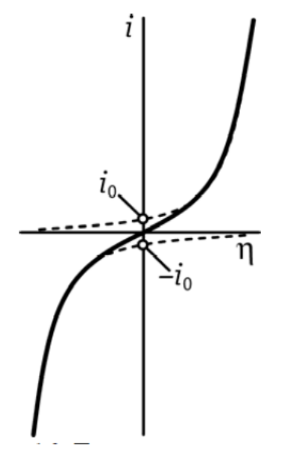
\includegraphics[width = 0.5\textwidth]{Б-Ф.png}
\caption{Поляризационная кривая стадии переноса заряда при $\alpha = 0,5$}
\label{fig:no_int}
\end{minipage}
\hfill
\begin{minipage}[h]{0.45\linewidth}
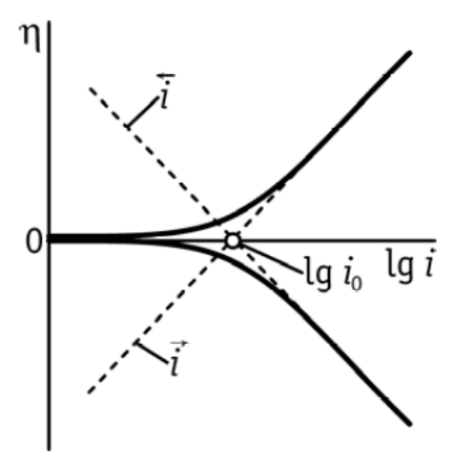
\includegraphics[width = 0.6\textwidth]{Тафель.png}
\caption{Поляризационная кривая в Тафелевских координатах}
\label{fig:no_int}
\end{minipage}
\end{center}
\end{figure}

\newpage
\section{Ход работы и обработка результатов}
\subsection{Получение и проверка работы хлорсеребрянных элетродов}
В данной части работы используется следующая трехэлетродная схема (ячейка заполнена 0.1M KCl):
\begin{itemize}
    \item Рабочий элетрод - Ag
    \item Противоэлектрод - Pt
    \item Электрод сравнения - хлорсеребрянный, заполненный 3.5М KCl
\end{itemize}
Проведем очистку хлорсеребрянного элетрода с помощью катодной поляризации в режиме линейной развертки потенциала от 0 до -1500мВ со скоростью 10мВ/с
\begin{figure}[h!]
    \centering
    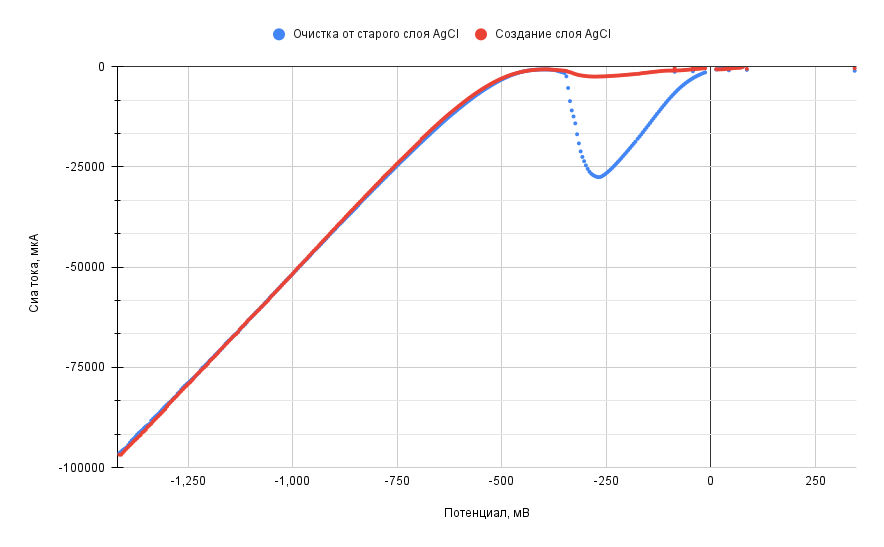
\includegraphics[width = 0.8\textwidth]{cleaning.png}
    \caption{ВАХ очистки элетрода}
    \label{fig:no_int}
\end{figure}\\
Рассмотрим первый проход. При малых отклонениях потенциала от равновесного на рабочем электроде идет следующая реакция восстановления:
\begin{equation*}
AgCl + e^- \rightarrow Ag + Cl^-
\end{equation*}

Далее ток снова становится равным 0. Это происходит из-за того, что весь AgCl уже восстановился, электрод стал серебрянным. При дальнейшем отклонении потенциала от равновесного происходит уже другая реакция, при которой наблюдается выделение газа:
\begin{equation*}
    e^{-}+ H_{2}O \rightarrow 1/2H_2 + OH^{-}\uparrow
\end{equation*}

График при этом быстро становится прямой, значит реация лимитирована диффузионно (потому что в этом случае малое фарадеевское сопротивление, и схема Эшлера - Рендлса примерно эквивалентна последовательно соединенным резисторам)\\
При втором проходе аналогичной первому проходу "ямы" не наблюдается. Это произошло потому, что при первом проходе весь AgCl "счистили" с электрода, а новому "нарасти" на дали (т.к. для этого надо провести анодную поляризацию)\\
Проведем анодную поляризацию очищенной серебрянной проволоки. При этом на рабочем электроде будет идти реакция окисления:
\begin{equation*}
 Ag + Cl^- - e^- \rightarrow AgCl
\end{equation*}
При проведении опыта действительно наблюдается "побурение" серебрянной проволоки.



\subsection{Поляризуемые и неполяризуемые электроды}
В данной части работы использовалась следующая трехэлектродная схема:
\begin{itemize}
    \item Рабочий электрод - Ag|AgCl и Pt
    \item Противоэлектрод - Pt
    \item Электрод сравнения - хлорсеребрянный
\end{itemize}
Измерим циклические ВАХ для рабочих электродов при скорости развертки 100 мВ/с и скорости регистрации - 13 точек/с по 5 циклов:
\begin{enumerate}
    \item Ag|AgCl электрода (от -150 до 150 мВ ) в растворе 1М KCl.
    \item Pt электрода (от -900 до 1150 мВ ) в растворе 1М KCl.
    \end{enumerate}

\begin{figure}[H]
    \centering
    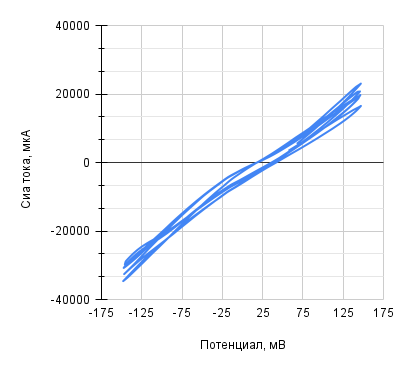
\includegraphics[width = 0.5\textwidth]{201.png}
    \caption{ЦВАХ Ag|AgCl электрода}
    \label{fig:no_int}
\end{figure}\\

\begin{figure}[H]
    \centering
    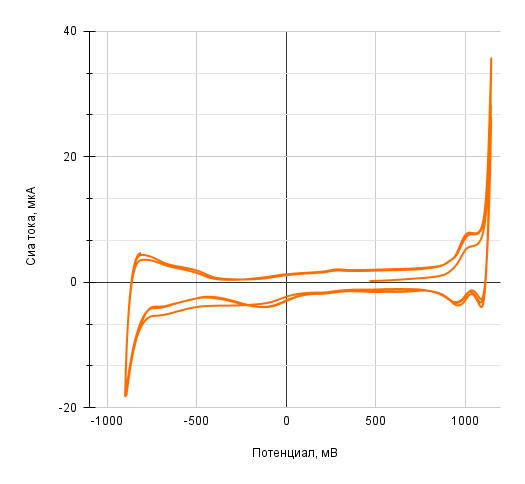
\includegraphics[width = 0.5\textwidth]{202.png}
    \caption{ЦВАХ Pt электрода}
    \label{fig:no_int}
\end{figure}\\

\begin{figure}[H]
    \centering
    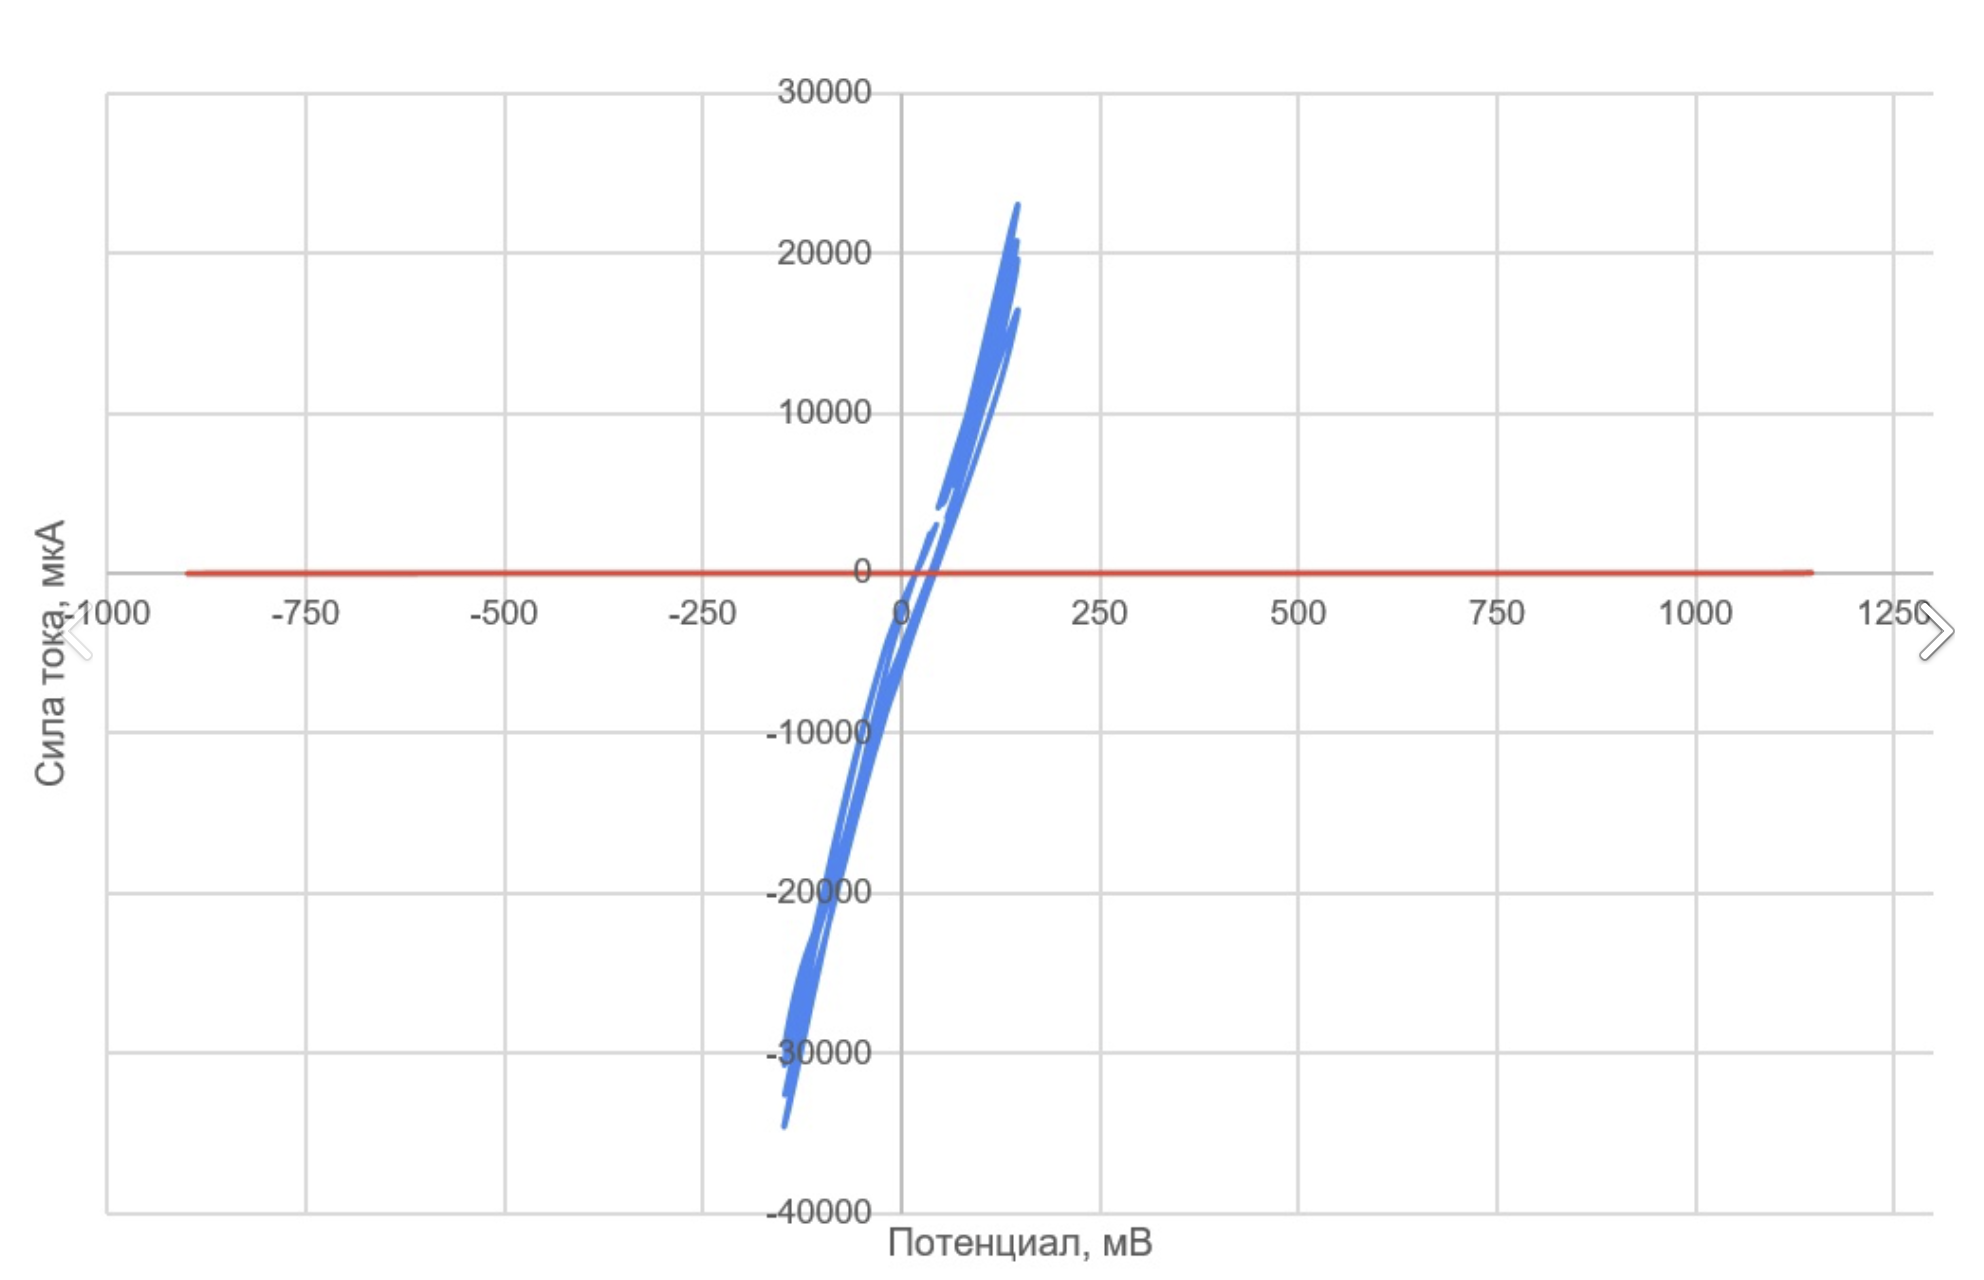
\includegraphics[width = 0.5\textwidth]{200.png}
    \caption{Сравнение ЦВАХ Ag|AgCl и Pt электродов}
    \label{fig:no_int}
\end{figure}\\

Как видно из полученных графиков, хлорсеребряный электрод - неполяризуемый, а платиновый - поляризуемый. \\
Процессы, происходящие на рабочих электродах
\begin{itemize}
    \item Хлорсеберянный электрод
    \begin{equation*}
        I_{anode} > 0 : Ag + Cl^- - e \rightarrow AgCl
    \end{equation*}
    \begin{equation*}
        I_{anode} < 0: AgCl + e \rightarrow Ag + Cl^-
    \end{equation*}
    \item Платиновый электрод
    \begin{equation*}
        I_{anode}> 0: Pt + H_2O \rightarrow Pt - O_{ads} + 2e(Pt) + 2H^+
    \end{equation*}
    \begin{equation*}
        I_{anode} < 0: H_3O^+ + e(Pt) \rightarrow Pt - H_{ads} + H_2O
    \end{equation*}
\end{itemize}
Видно, что Pt электрод является идеально поляризуемым в диапазоне [0, 750mV] относительно хлорсеребрянного электрода. 


\newpage

\subsection{Стационарые кривые поляризации для Ox-Red электрода}
В данной части работы были получены кривые поляризации рабочего Pt электрода (3х электродная схема) при различных концентрациях  $K_3[Fe(CN)_6]$ и одинаковой скорости перемешивания. Исходные концентрации $C(K_4[Fe(CN)_6]) = C(K_4[Fe(CN)_6]) = 1.923 мM$

\begin{table}[h!]
\centering{%
\begin{tabular}{|c|c|c|c|c|}
\hline
$V_{K4}, \mbox{мл} $ & $V_{K3}, \mbox{мл}$ & $V_{\text {общ }},$ мл & $C_{K4},\mbox{мМ}$ & $C_{K3}, \mbox{мМ}$ \\ \hline
1 & 1 & 52 & 1.923 & 1.923 \\ \hline
1 & 3 & 54 & 1.852 & 5.556 \\ \hline
1 & 5 & 56 & 1.786 & 8.929 \\ \hline
1 & 7 & 58 & 1.724 & 12.069 \\ \hline
1 & 9 & 60 & 1.667 & 15.000 \\ \hline
1 & 11 & 62 & 1.613 & 17.742 \\ \hline
\end{tabular}%
}
\caption{Концентрация $K_{3}[Fe(CN)_{6}]$, $K_{4}[Fe(CN)_{6}]$}

\label{tab:my-table}
\end{table}
\begin{figure}[h!]
    \centering
    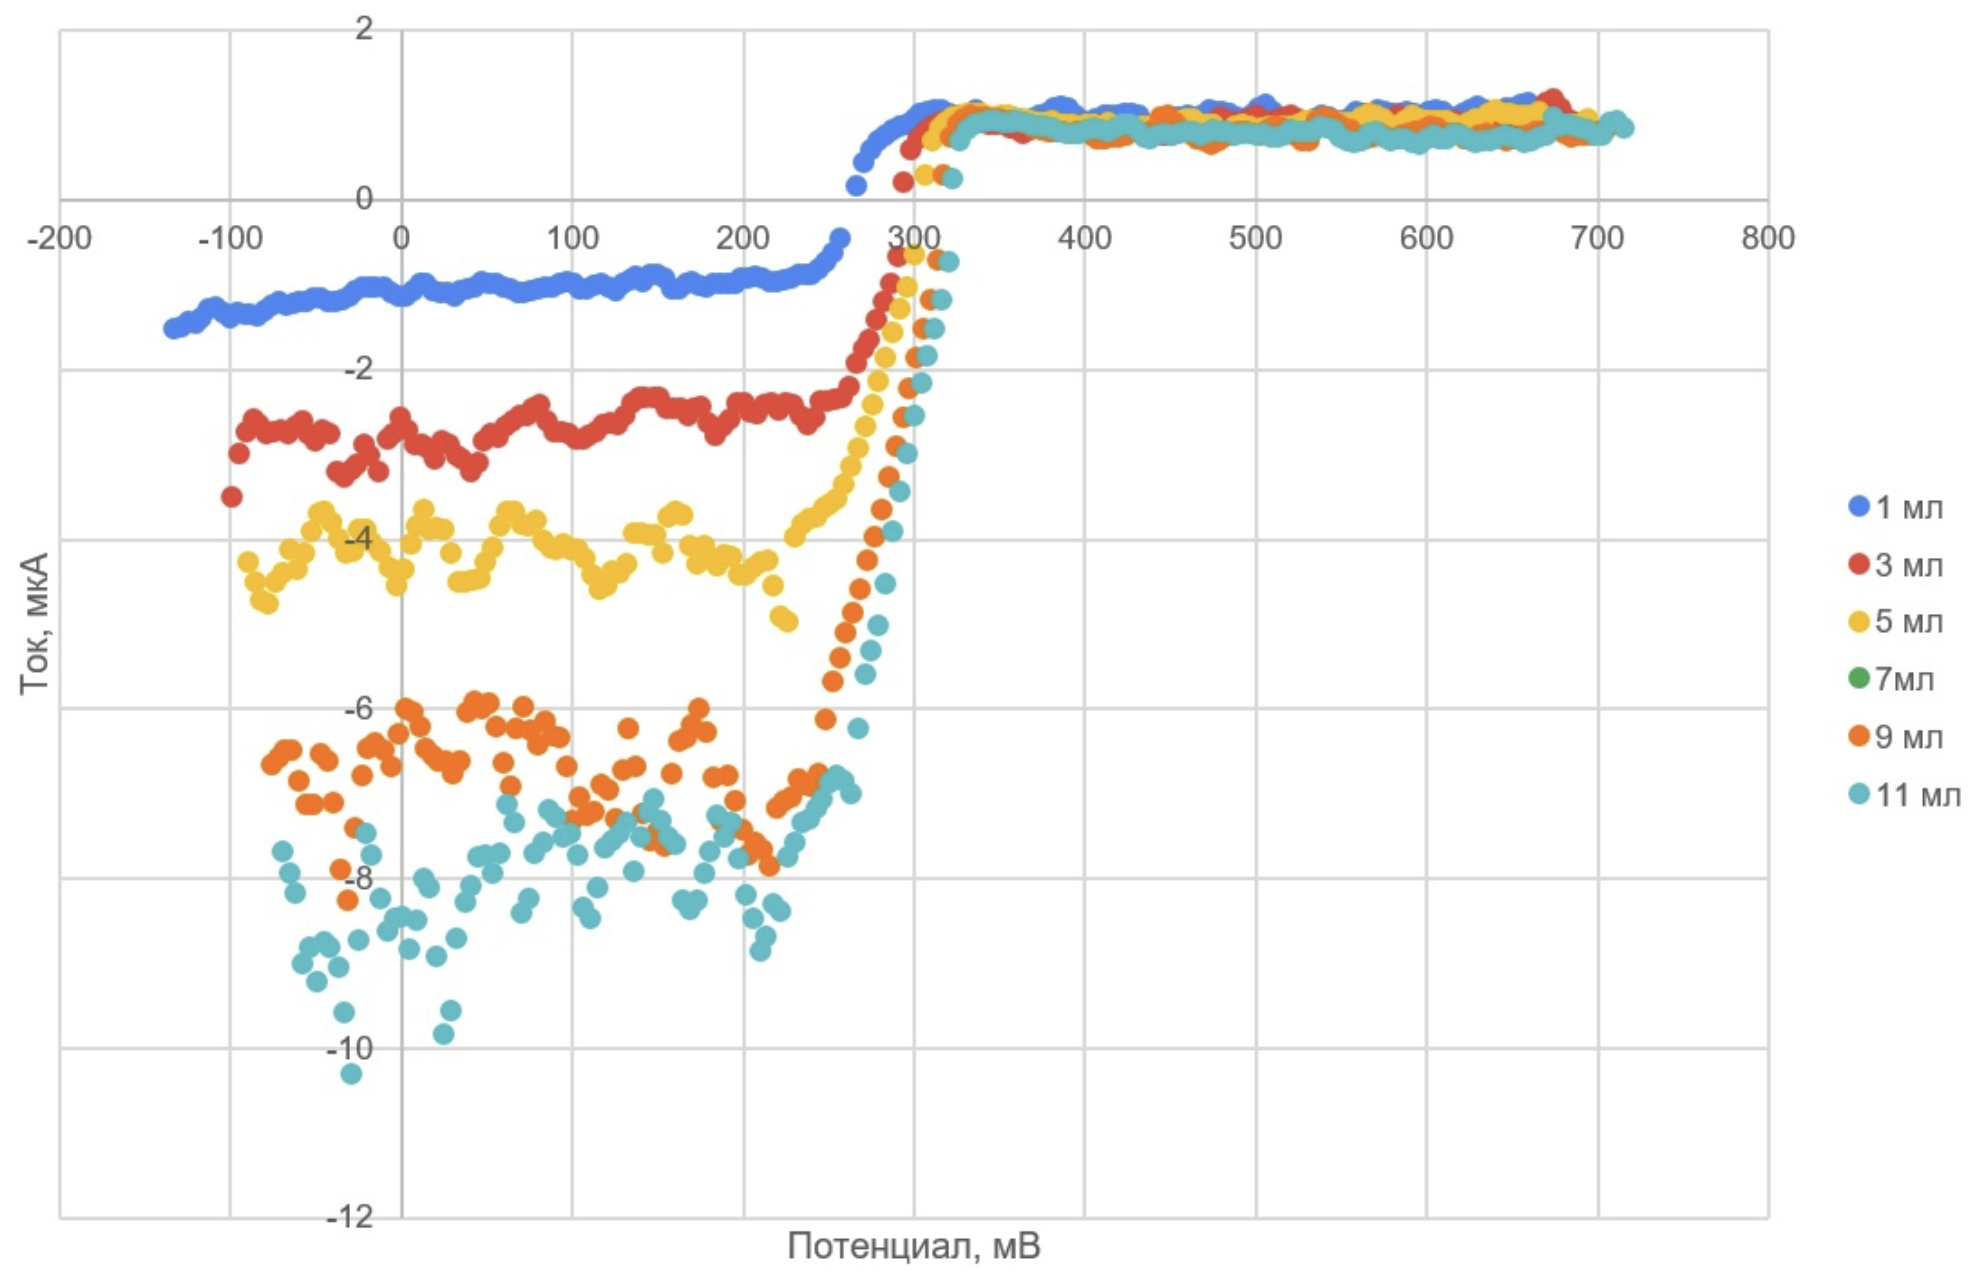
\includegraphics[width = 0.8\textwidth]{changes in conc.png}
    \caption{Кривые поляризации Pt электрода при различной концентрации $C(K_4[Fe(CN)_6])$}
    \label{fig:no_int}
\end{figure}\\

Процессы, идущие на рабочем электроде:
\begin{equation*}
    I_{anode} < 0: [Fe(CN)_6]^{3-} + e^- \rightarrow [Fe(CN)_6]^{4-}
\end{equation*}
\begin{equation*}
    I_{anode} > 0: [Fe(CN)_6]^{4-} - e^- \rightarrow [Fe(CN)_6]^{3-}
\end{equation*}

Поскольку ток ограничен для обоих процессов, делаем вывод, что диффузия лимитирует как окисление, так и восстановление. Предельный диффузионный ток восстановленной формы остается постоянным в отличие от тока окисленной формы($K_3[Fe(CN)_6]$).\\
\text{Катодная поляризация}: $[Fe(CN)_6]^{3-} + e^- \rightarrow [Fe(CN)_6]^{4-} $ \\
$E < E_{\text{р}}$, процесс лимитирован диффузией окисленной формы, концентрация которой значительно меняется в ходе эксперимента\\\\
\text{Анодная поляризация}: $[Fe(CN)_6]^{4-} - e^- \rightarrow [Fe(CN)_6]^{3-}$\\
$E > E_{\text{р}}$, процесс лимитирован диффузией восстановленной формы, концентрация которой  меняется в ходе эксперимента незначительно.\\
\begin{figure}[h!]
    \centering
    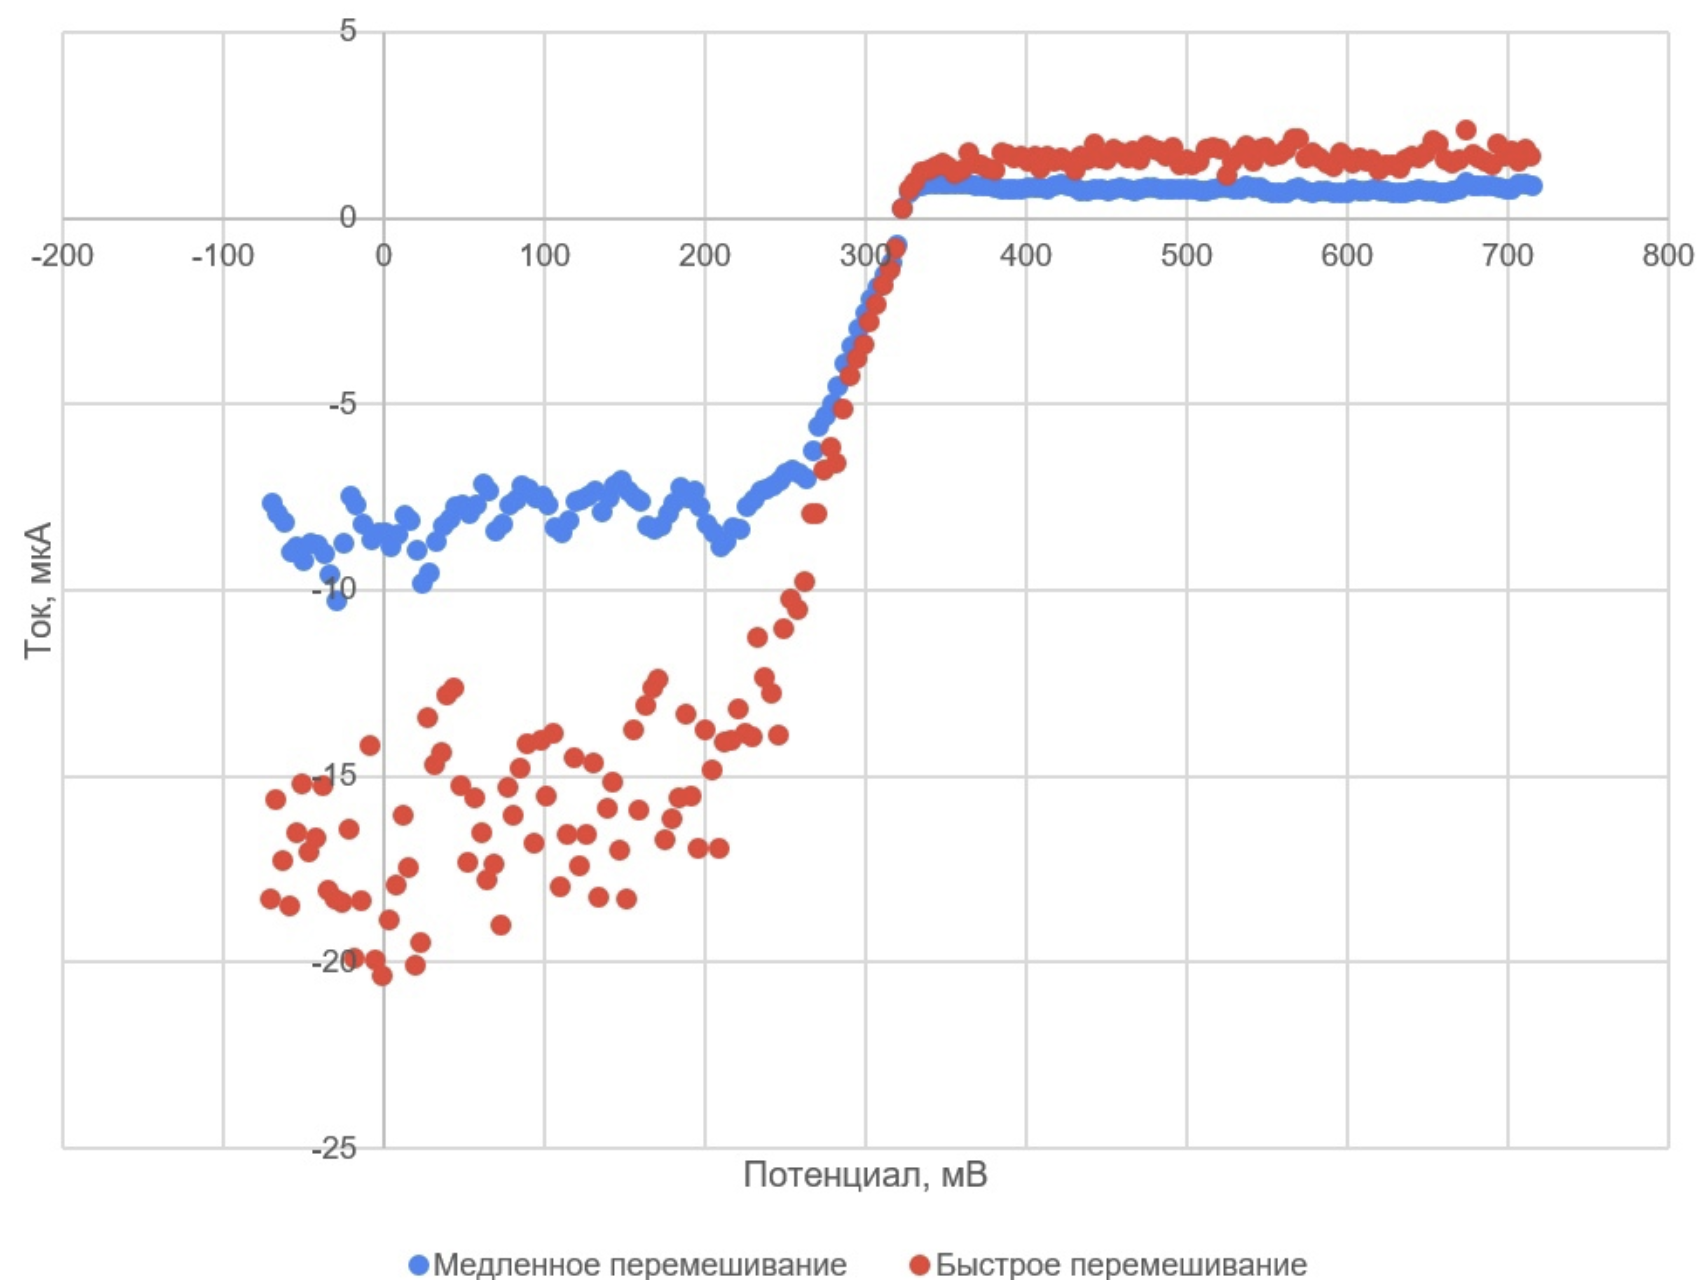
\includegraphics[width = 0.5\textwidth]{pace.png}
    \caption{Кривые поляризации Pt электрода при быстром\\
и медленном перемешивании}
    \label{fig:no_int}
\end{figure}\\


\\
\begin{table}[h!]
\centering{%
\begin{tabular}{|c|c|c|c|c|}
\hline
$V_{K4}, \mbox{мл} $ & $V_{K3}, \mbox{мл}$ & $V_{\text {общ }},$ мл & $C_{K4},\mbox{мМ}$ & $C_{K3}, \mbox{мМ}$ \\ \hline
1 & 1 & 62 & 1.61 & 1.61 \\ \hline
1 & 3 & 64 & 1.56 & 4.69 \\ \hline
1 & 5 & 66 & 1.52 & 7.58 \\ \hline
1 & 7 & 68 & 1.47 & 10.29 \\ \hline
1 & 9 & 70 & 1.43 & 12.86 \\ \hline
\end{tabular}%
}
\caption{Концентрация $K_{3}[Fe(CN)_{6}]$}
\label{tab:my-table}
\end{table}


Придерживаясь {IUPAC}:\\
$$i^{ Ox }= - n F D \frac{(c ^ b - c ^ s)}{\delta},\hspace{10}$$
$$i^{ Ox }_{d}= -n F D \frac{c ^ b}{\delta},\hspace{10}$$\\
$i^{Ox}_d$ - предельный диффузионный ток на единицу площади окисленной формы, $D$ - коэффициент диффузии, $c ^ s$ - поверхностная концентрация  ионов при катодном токе, $\delta$- толщина диффузионного слоя\\
Оценим толщину диффузионного слоя по значениям предельного катодного тока при разных концентрациях $K_3[Fe(CN)_6]$. Для этого построим график $i_d (C)$. По коэффициенту наклона графика найдем $\delta$ (S - площадь поверхности электрода):\\
$$k = -nFDS/ \delta$$
$$k = - 4,3695*10^-^6 A m^3/mol$$
$$D = 8,96*10^-^1^0{m^2/c}$$

\begin{table}[h!]
\begin{center}{%
\begin{tabular}{|c|c|}
\hline
\textbf{$C_{K3}, \mbox{мМ}$} & \textbf{$i_d (C)$} \\ \hline
1.923 & -1.05 \\ \hline
5.556 & -2.72 \\ \hline
8.929 & -4.14 \\ \hline
12.069 & -5.5 \\ \hline
15.000 & -6.66 \\ \hline
17.742 & -8.08 \\ \hline
\end{tabular}%
}
\caption{Предельный катодный ток при разных концентрациях $K_3[Fe(CN)_6]$}
\label{tab:my-table}
\end{center}
\end{table}

\begin{figure}[h!]
    \centering
    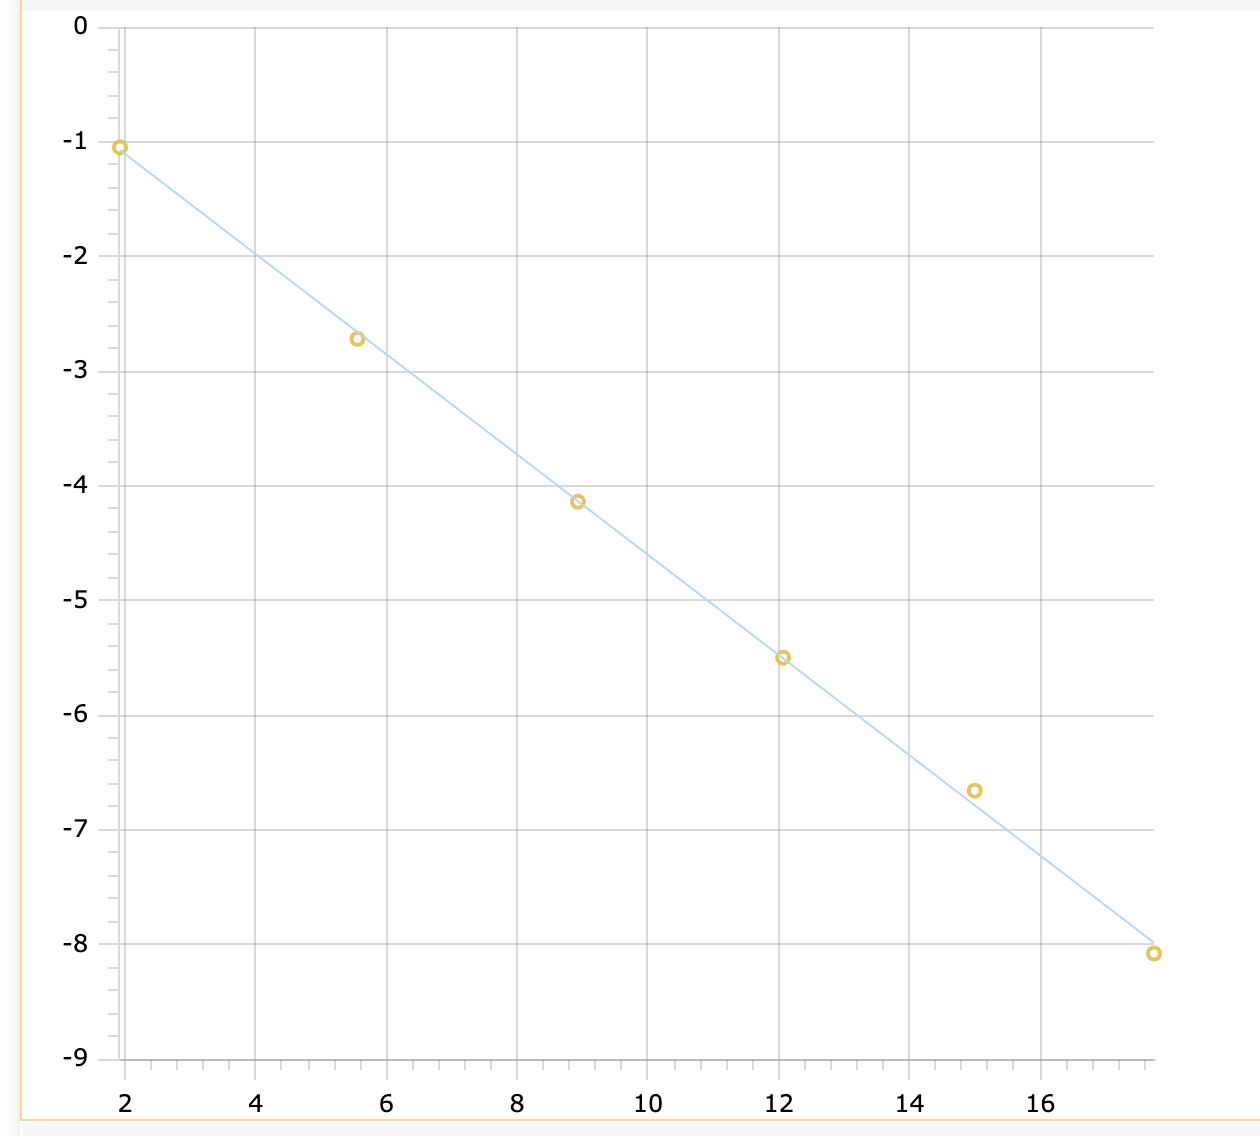
\includegraphics[width = 0.5\textwidth]{300.png}
    \caption{Зависимость предельного диффузионного тока от концентрации}
    \label{fig:no_int}
\end{figure}\\


Площадь поверхности электрода (длина электрода l = 1мм, радиус r = 0.5мм):
\begin{equation*}
    S = 2 \pi rh + \pi r^2 = 4 \cdot 10^{-6} m^2
\end{equation*}
$$
\delta = \frac{FDS}{k} = 79,14 \text{ мкм}
$$

Оценим количество электронов, задействованных в реакции.\\
Стационартный потенциал электрода - при i = 0. Тогда равны концентрации $c^b$ соли в объеме вещества и $c^s$ на внутренней границе диффузионного слоя (т.к. $i \sim C^s - C^b$). Тогда из уравнения Нернста:
\begin{equation*}
    E_p = E_0 + \frac{RT}{nF}\ln{\frac{C^s[Fe(CN)_6]^{3-}}{C^s([Fe(CN)_6]^{4-})}} =  E_0 + \frac{RT}{nF}\ln{\frac{C^b[Fe(CN)_6]^{3-}}{C^b([Fe(CN)_6]^{4-})}}
\end{equation*}
% Please add the following required packages to your document preamble:
% \usepackage{graphicx}
\begin{table}[h!]
\centering
{%
\begin{tabular}{|c|c|r|r|}
\hline
C_{K3} & C_{K3} & \multicolumn{1}{c|}{$\ln ({C_{4-})} /{C_{3-})} )$} & \multicolumn{1}{c|}{$\mbox{E_p}, \mbox{мВ}$} \\ \hline
1.923 & 1.923 & 0.000 & 264.15 \\ \hline
1.852 & 5.556 & -1.099 & -294.67 \\ \hline
1.786 & 8.929 & -1.609 & 312.91 \\ \hline
1.724 & 12.069 & -1.946 & 320.87 \\ \hline
1.667 & 15.000 & -2.197 & 324.22 \\ \hline
1.613 & 17.742 & -2.398 & 325.57 \\ \hline
\end{tabular}%
}
\caption{Зависимость Ep от логарифма отношения концентраций}
\label{tab:my-table}
\end{table}

\begin{figure}[h!]
    \centering
    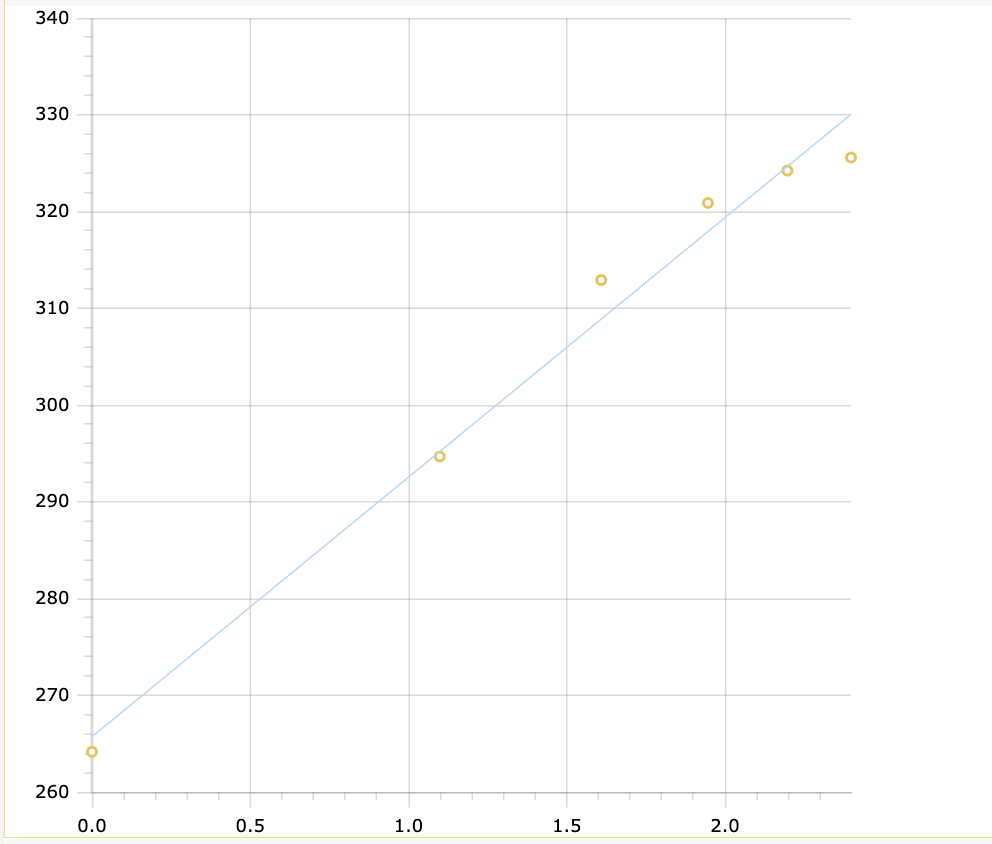
\includegraphics[width = 0.4\textwidth]{301.png}
    \caption{Зависимость стационарного потенциала электрода от логарифма отношения концентраций солей}
    \label{fig:no_int}
\end{figure}\\

Значит, $k = 26.827 мВ$. Тогда число электронов:
\begin{equation*}
    k = \frac{RT}{nF} \Rightarrow n = \frac{RT}{kF} = \frac{8.31 \cdot 298}{26.827 \cdot 10^{-3} \cdot 96485} = 1.01\approx 1
\end{equation*}
Таким образом, в одной реации задействован примерно один электрон (что подтверждает исходное уравнение реакции). \\
\section{Выводы}
\begin{itemize}
\item Хлорсеребряный электрод является идеально неполяризуемым в пределах [-150, 150mV]
\itemПлатиновый электрод можно считать идельно поляризуемым в диапазоне [-700, 800mV]\\
\itemТолщина неперемешиваемого слоя Pt электрода в присутствии ферроцианида и феррицианида калия $\delta = 79, 14 $ мкм.Она уменьшается при усиленном перемешивании.\\ 
\itemНа один ион феррицианида приходится один электрон.
\end{itemize}





\end{document}